\documentclass[8pt,a4paper,compress]{beamer}

\usepackage{/home/siyer/lib/slides}

\title{Balanced Search Trees}
\date{}

\begin{document}
\begin{frame}
\vfill
\titlepage
\end{frame}

\begin{frame}
\frametitle{Outline}
\tableofcontents
\end{frame}

\section{2-3 Search Trees}
\begin{frame}[fragile]
\begin{itemize}
\item a 2-3 search tree is a tree that is either empty (null link) or
\begin{itemize}
\item a 2-node with one key (and associated value) and two links, a left link to a 2-3 search tree with smaller keys, and a right link to a 2-3 search tree with larger keys

\item a 3-node with two keys (and associated values) and three links, a left link to a 2-3 search tree with smaller keys, a middle link to a 2-3 search tree with keys between the node's keys, and a right link to a 2-3 search tree with larger keys
\end{itemize}

\begin{center}
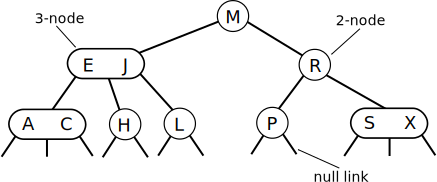
\includegraphics[scale=0.4]{{./figures/23_tree}.png}
\end{center}

\item a 2-3 search tree has symmetric order --- inorder traversal yields keys in ascending order

\item a perfectly balanced 2-3 search tree is one whose null links are all the same distance from the root

\begin{center}
\includegraphics[scale=0.3]{{./figures/23_tree_perfect_balance}.png}
\end{center}
\end{itemize}
\end{frame}

\begin{frame}[fragile]
\begin{itemize}
\item searching for a key in a 2-3 tree
\begin{center}
\includegraphics[scale=0.4]{{./figures/23_tree_search}.png}

\smallskip

\small search hit (left) and search miss (right) in a 2-3 tree
\end{center}
\end{itemize}
\end{frame}

\begin{frame}[fragile]
\begin{itemize}
\item inserting into a 2-3 tree
\begin{itemize}
\item insert into a 2-node
\begin{center}
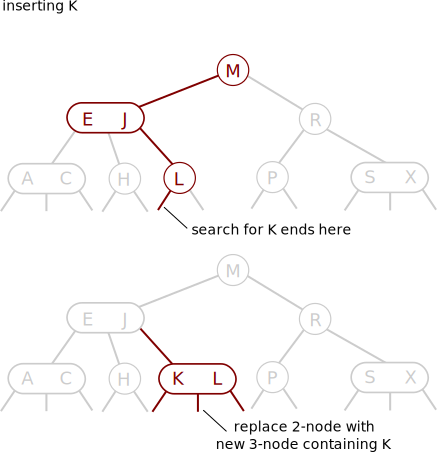
\includegraphics[scale=0.4]{{./figures/23_tree_insert1}.png}
\end{center}

\item insert into a single 3-node
\begin{center}
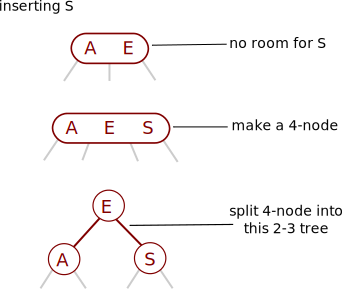
\includegraphics[scale=0.4]{{./figures/23_tree_insert2}.png}
\end{center}
\end{itemize}
\end{itemize}
\end{frame}

\begin{frame}[fragile]
\begin{itemize}
\item inserting into a 2-3 tree (contd.)
\begin{itemize}
\item insert into a 3-node whose parent is a 2-node
\begin{center}
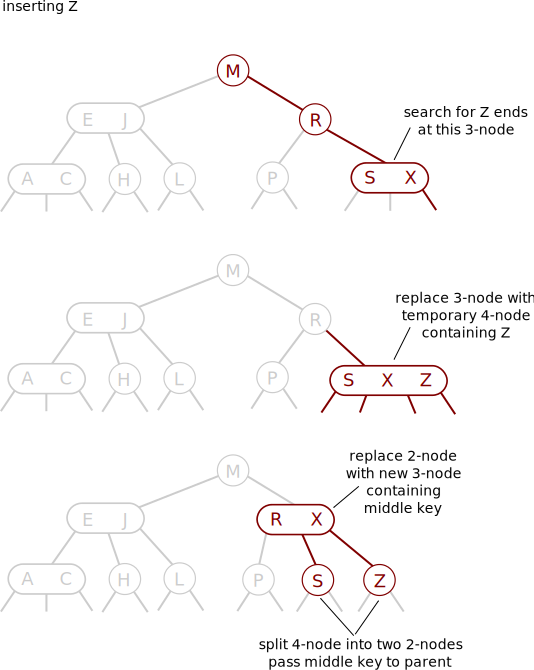
\includegraphics[scale=0.4]{{./figures/23_tree_insert3}.png}
\end{center}
\end{itemize}
\end{itemize}
\end{frame}

\begin{frame}[fragile]
\begin{itemize}
\item inserting into a 2-3 tree (contd.)
\begin{itemize}
\item insert into a 3-node whose parent is a 3-node
\begin{center}
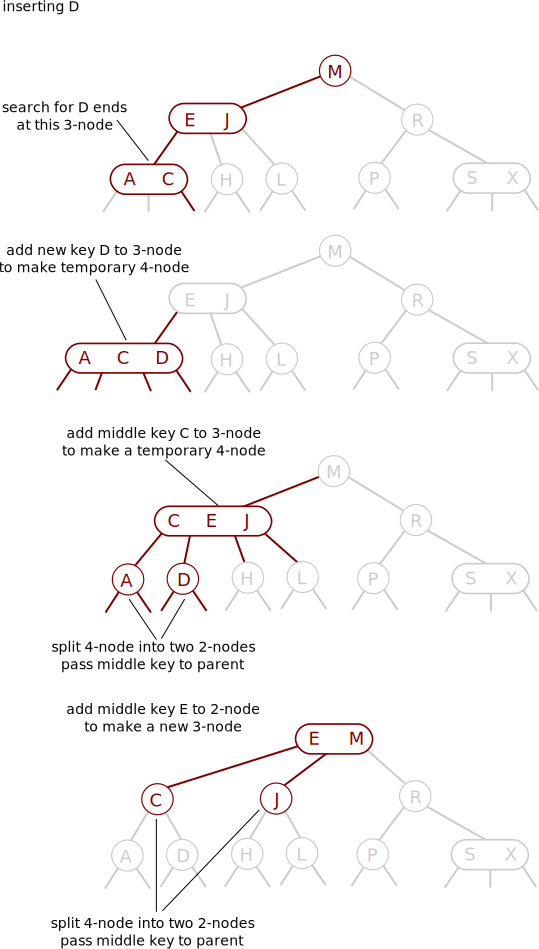
\includegraphics[scale=0.4]{{./figures/23_tree_insert4}.png}
\end{center}
\end{itemize}
\end{itemize}
\end{frame}

\begin{frame}[fragile]
\begin{itemize}
\item inserting into a 2-3 tree (contd.)
\begin{itemize}
\item splitting the root
\begin{center}
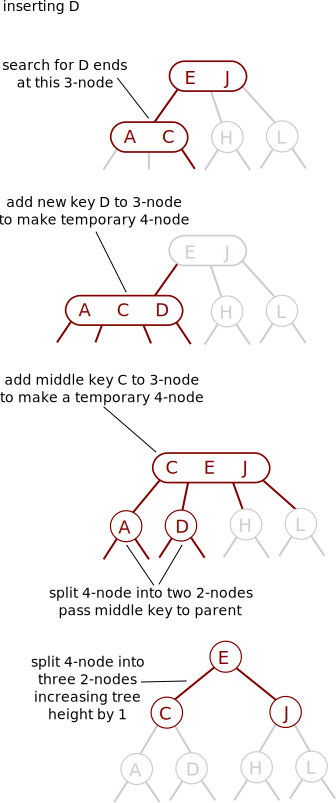
\includegraphics[scale=0.4]{{./figures/23_tree_insert5}.png}
\end{center}
\end{itemize}
\end{itemize}
\end{frame}

\begin{frame}[fragile]
\begin{itemize}
\item splitting a 4-node is a local transformation: constant number of operations

\item insert operation maintains symmetric order and perfect balance

\item tree height
\begin{itemize}
\item worst case: $\lg N$ (all 2-nodes)

\item best case: $\log_3 N \approx 0.631 \lg N$ (all 3-nodes)

\item between 12 and 20 for a million nodes

\item between 18 and 30 for a billion nodes
\end{itemize}

\item guaranteed logarithmic performance for search and insert
\end{itemize}
\end{frame}

\begin{frame}[fragile]
\begin{itemize}
\item direct implementation is complicated because:
\begin{itemize}
\item maintaining multiple node types is cumbersome

\item need multiple comparisons to move down tree

\item need to move back up the tree to split 4-nodes

\item large number of cases for splitting
\end{itemize}

\smallskip

fantasy code:
\begin{lstlisting}[language=Java]
public void put(Key key, Value val) {
    Node x = root;
    while (x.getTheCorrectChild(key) != null) {
        x = x.getTheCorrectChildKey();
        if (x.is4Node()) { x.split(); }
    }
    if (x.is2Node()) { x.make3Node(key, val); }
    else if (x.is3Node()) { x.make4Node(key, val); }
}
\end{lstlisting}

could do it, but there's a better way (use red-black BSTs)
\end{itemize}
\end{frame}

\section{Red-Black BSTs}
\begin{frame}[fragile]
\begin{itemize}
\item represent a 2-3 tree as a BST, using ``internal'' left-leaning links as ``glue'' for 3-nodes

\begin{center}
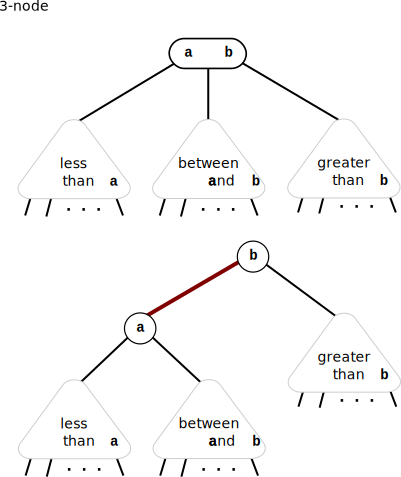
\includegraphics[scale=0.4]{{./figures/red_black_bst1}.png}
\end{center}

\item a red-black tree is a BST such that:
\begin{itemize}
\item no node has two red links connected to it

\item every path from root to null link has the same number of black links (perfect black balance)

\item red links lean left
\end{itemize}

\begin{center}
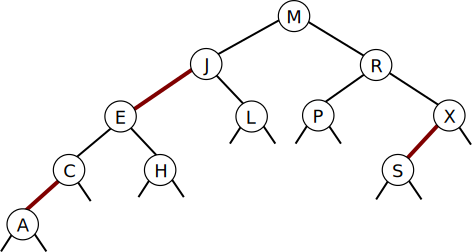
\includegraphics[scale=0.4]{{./figures/red_black_bst2}.png}
\end{center}
\end{itemize}
\end{frame}

\begin{frame}[fragile]
\begin{itemize}
\item 1-1 correspondence between red-black BSTs and 2-3 trees

\begin{center}
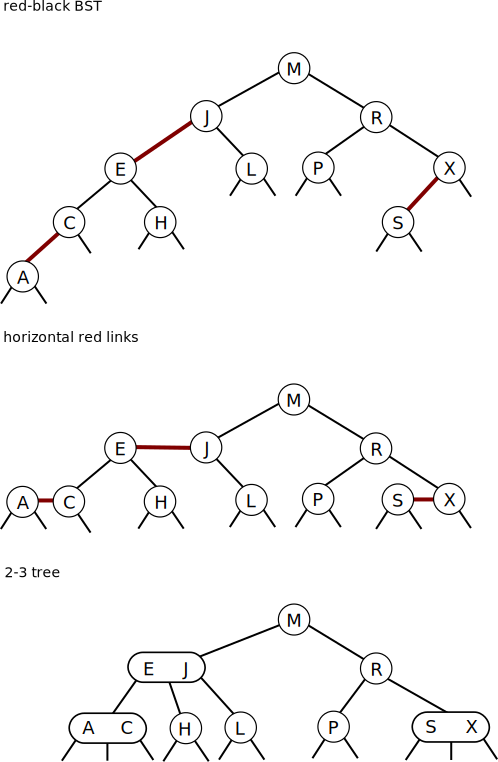
\includegraphics[scale=0.4]{{./figures/red_black_bst3}.png}
\end{center}
\end{itemize}
\end{frame}

\begin{frame}[fragile]
\begin{itemize}
\item red-black BST representation: each node is pointed to by precisely one link (from its parent) $\implies$ can encode color of links in nodes

\begin{minipage}{180pt}
\begin{lstlisting}[language=Java]
...
    private static final boolean RED   = true;
    private static final boolean BLACK = false;

    private class Node {
        private Key key;
        private Value val;
        private Node left, right; 
        private boolean color; 
        private int N;

        public Node(Key key, Value val, 
                    boolean color, int N) {
           this.key = key;
           this.val = val;
           this.color = color;
           this.N = N;
        }
    }
    
    private boolean isRed(Node x) {
        if (x == null) { return false };
        return x.color == RED;
    }
...
\end{lstlisting}
\end{minipage}%
\begin{minipage}{100pt}
\begin{center}
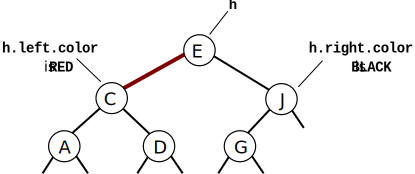
\includegraphics[scale=0.4]{{./figures/red_black_bst4}.png}
\end{center}
\end{minipage}
\end{itemize}
\end{frame}

\begin{frame}[fragile]
\begin{itemize}
\item elementary red-black BST operations
\begin{itemize}
\item left rotation: orient a (temporarily) right-leaning red link to lean left
\begin{minipage}{170pt}
\begin{lstlisting}[language=Java]
private Node rotateLeft(Node h) {
    Node x = h.right;
    h.right = x.left;
    x.left = h;
    x.color = x.left.color;
    x.left.color = RED;
    x.N = h.N;
    h.N = size(h.left) + size(h.right) + 1;
    return x;
}
\end{lstlisting}
\end{minipage}%
\begin{minipage}{100pt}
\begin{center}
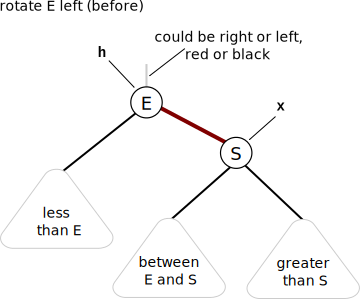
\includegraphics[scale=0.4]{{./figures/red_black_bst5}.png}

\smallskip

rotate E left (before)
\end{center}
\begin{center}
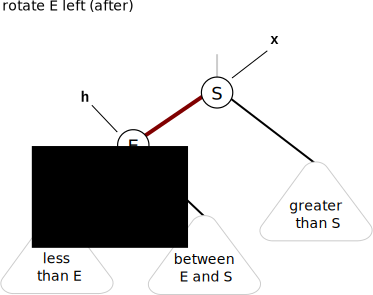
\includegraphics[scale=0.4]{{./figures/red_black_bst6}.png}

\smallskip

rotate E left (after)
\end{center}
\end{minipage}

\item maintains symmetric order and perfect black balance
\end{itemize}
\end{itemize}
\end{frame}

\begin{frame}[fragile]
\begin{itemize}
\item elementary red-black BST operations (contd.)
\begin{itemize}
\item right rotation: orient a left-leaning red link to (temporarily) lean right
\begin{minipage}{170pt}
\begin{lstlisting}[language=Java]
private Node rotateRight(Node h) {
    Node x = h.left;
    h.left = x.right;
    x.right = h;
    x.color = x.right.color;
    x.right.color = RED;
    x.N = h.N;
    h.N = size(h.left) + size(h.right) + 1;
    return x;
}
\end{lstlisting}
\end{minipage}%
\begin{minipage}{100pt}
\begin{center}
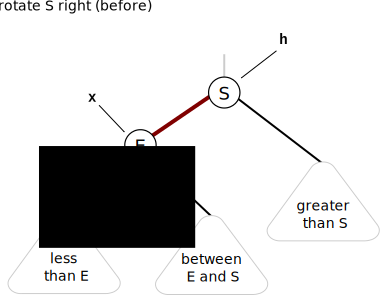
\includegraphics[scale=0.4]{{./figures/red_black_bst7}.png}

\smallskip

rotate S right (before)
\end{center}
\begin{center}
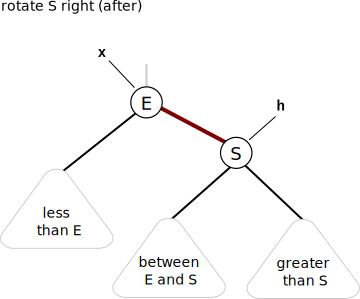
\includegraphics[scale=0.4]{{./figures/red_black_bst8}.png}

\smallskip

rotate S right (after)
\end{center}
\end{minipage}

\item maintains symmetric order and perfect black balance
\end{itemize}
\end{itemize}
\end{frame}

\begin{frame}[fragile]
\begin{itemize}
\item elementary red-black BST operations (contd.)
\begin{itemize}
\item color flip: recolor to split a (temporary) 4-node
\begin{minipage}{170pt}
\begin{lstlisting}[language=Java]
private void flipColors(Node h) {
    h.color = !h.color;
    h.left.color = !h.left.color;
    h.right.color = !h.right.color;
}
\end{lstlisting}
\end{minipage}%
\begin{minipage}{100pt}
\begin{center}
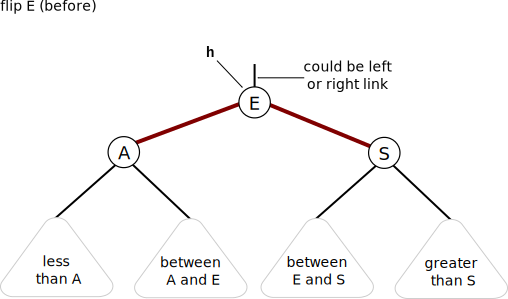
\includegraphics[scale=0.4]{{./figures/red_black_bst9}.png}

\smallskip

flip colors (before)
\end{center}
\begin{center}
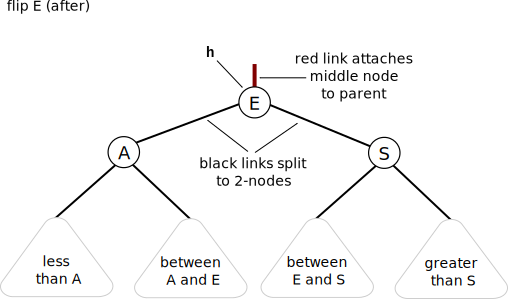
\includegraphics[scale=0.4]{{./figures/red_black_bst10}.png}

\smallskip

flip colors (after)
\end{center}
\end{minipage}

\item maintains symmetric order and perfect black balance
\end{itemize}
\end{itemize}
\end{frame}

\section{Implementation of the Ordered Symbol Table API Using a Red-Black BST}
\begin{frame}[fragile]
\begin{itemize}
\item most operations are the same as for BST-based implementation --- ignore color
\begin{lstlisting}[language=Java]
import java.util.NoSuchElementException;

public class RedBlackTreeST<Key extends Comparable<Key>, Value> implements 
    OrderedST<Key, Value> {
    private Node root;  
    ...    
    public boolean isEmpty() { ... }

    public int size() { ... }

    public Value get(Key key) { ... }

    public boolean contains(Key key) { ... }

    public Key min() { ... } 

    public Key max() { ... } 

    public Key floor(Key key) { ... }
    
    public Key ceiling(Key key) { ... }

    public int rank(Key key) { ... } 

    public Key select(int k) { ... }
    
    public int size(Key lo, Key hi) { ... }
    
    public Iterable<Key> keys() { ... }

    public Iterable<Key> keys(Key lo, Key hi) { ... }
    ...
}
\end{lstlisting}
\end{itemize}
\end{frame}

\begin{frame}[fragile]
\begin{itemize}
\item insertion: the basic strategy is to maintain 1-1 correspondence with 2-3 trees, using the elementary red-black BST operations (left/right rotation and color flip) to maintain symmetric order and perfect balance, but not necessarily color invariants

\begin{itemize}
\item case 1 (insert into a 2-node at the bottom): do standard BST insert; color new link red; if new red link is a right link, rotate left

\begin{center}
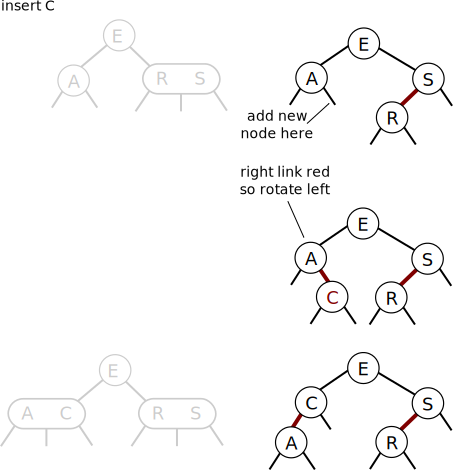
\includegraphics[scale=0.4]{{./figures/red_black_bst11}.png}
\end{center}
\end{itemize}
\end{itemize}
\end{frame}

\begin{frame}[fragile]
\begin{itemize}
\item insertion (contd.)
\begin{itemize}
\item case 2 (insert into a 3-node at the bottom): do standard BST insert; color new link red; rotate to balance the 4-node (if needed); flip colors to pass red link up one level; rotate to make lean left (if needed); repeat case 1 or case 2 up the tree (if needed)

\begin{center}
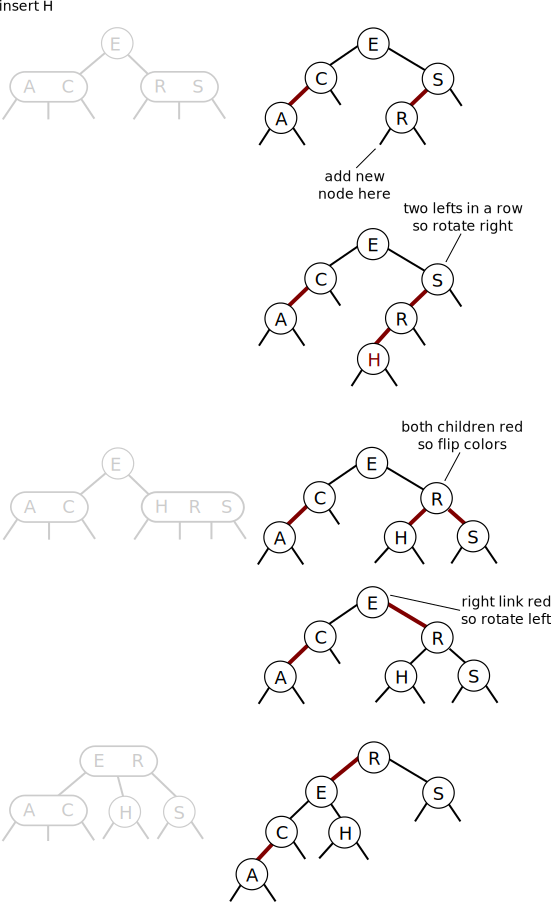
\includegraphics[scale=0.35]{{./figures/red_black_bst12}.png}
\end{center}
\end{itemize}
\end{itemize}
\end{frame}

\begin{frame}[fragile]
\begin{itemize}
\item insertion (contd.)
\begin{minipage}{150pt}
implementation (same code for all cases): 
\begin{itemize}
\item right child red, left child black: rotate left

\item left child, left-left grandchild red: rotate right

\item both children red: flip colors
\end{itemize}
\end{minipage}%
\begin{minipage}{100pt}
\begin{center}
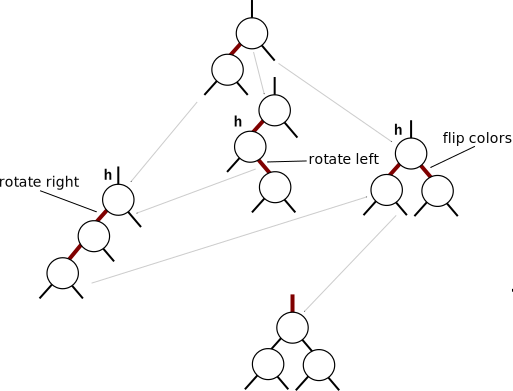
\includegraphics[scale=0.35]{{./figures/red_black_bst13}.png}
\end{center}
\end{minipage}

\begin{lstlisting}[language=Java]
    ...
    public void put(Key key, Value val) {
        root = put(root, key, val);
        root.color = BLACK;
    }

    private Node put(Node h, Key key, Value val) { 
        if (h == null) { return new Node(key, val, RED, 1); }
        int cmp = key.compareTo(h.key);
        if      (cmp < 0) { h.left  = put(h.left,  key, val); }
        else if (cmp > 0) { h.right = put(h.right, key, val); }
        else              { h.val   = val; }
        if (isRed(h.right) && !isRed(h.left))      { h = rotateLeft(h); }
        if (isRed(h.left)  &&  isRed(h.left.left)) { h = rotateRight(h); }
        if (isRed(h.left)  &&  isRed(h.right))     { flipColors(h); }
        h.N = size(h.left) + size(h.right) + 1;
        return h;
    }
    ...
\end{lstlisting}
\end{itemize}
\end{frame}

\begin{frame}[fragile]
\begin{itemize}
\item deletion: see exercises 3.3.39 -- 3.3.41

\item the height of a red-black BST with $N$ nodes is no more than $2 \lg N$; the average length of a path from the root to a node in a red-black BST with $N$ nodes is $\sim \lg N$

\begin{center}
\includegraphics[scale=0.35]{{./figures/red_black_bst14}.png}

\smallskip

\small typical red-black BST built from random keys (null links omitted)
\end{center}

\begin{center}
\includegraphics[scale=0.35]{{./figures/red_black_bst15}.png}

\smallskip

\small red-black BST built from ascending keys (null links omitted)
\end{center}
\end{itemize}
\end{frame}

\section{Performance Characteristics}
\begin{frame}[fragile]
\begin{itemize}
\item symbol table operations summary

\begin{center}
\begin{tabular}{ccc}
\textbf{operation} & \textbf{BST} & \textbf{red-black BST} \\ \hline \\
search & $h^\dagger$ & $2\lg N$ \\
insert & $h$ & $2\lg N$ \\
delete & $N^{\dagger\dagger}$ & $2\lg N$ \\
min/max & $h$ & $2\lg N$ \\
floor/ceiling & $h$ & $2\lg N$ \\
rank & $h$ & $2\lg N$ \\
select & $h$ & $2\lg N$ \\
ordered iteration & $N$ & $N$ 
\end{tabular}

\bigskip

\tiny $\dagger$ $h$ is the height of BST, proportional to $\lg N$ if keys inserted in random order

$\dagger\dagger$ $\sqrt{N}$ in the average case; other operations also become $\sqrt{N}$ if deletions are allowed
\end{center} 
\end{itemize}
\end{frame}

\end{document}
